\documentclass[notes,11pt, aspectratio=169]{beamer}

\usepackage{pgfpages}
\setbeameroption{hide notes} % Only slide

\usepackage{array}
\usepackage{tikz}
\usepackage{verbatim}
\setbeamertemplate{note page}{\pagecolor{gray!5}\insertnote}
\usetikzlibrary{positioning}
\usetikzlibrary{snakes}
\usetikzlibrary{calc}
\usetikzlibrary{arrows}
\usetikzlibrary{decorations.markings}
\usetikzlibrary{shapes.misc}
\usetikzlibrary{matrix,shapes,arrows,fit,tikzmark}
\usepackage{amsmath}
\usepackage{mathpazo}
\usepackage{hyperref}
\usepackage{lipsum}
\usepackage{multimedia}
\usepackage{graphicx}
\usepackage{multirow}
\usepackage{dcolumn}
\usepackage{bbm}
\newcolumntype{d}[0]{D{.}{.}{5}}

\usepackage{changepage}
\usepackage{appendixnumberbeamer}

\usepackage[space]{grffile}
\usepackage{booktabs}

% Colors
\definecolor{blue}{RGB}{0,114,178}
\definecolor{red}{RGB}{213,94,0}
\definecolor{yellow}{RGB}{240,228,66}
\definecolor{green}{RGB}{0,158,115}
\definecolor{solutionbg}{RGB}{240,248,240}
\definecolor{solutionframe}{RGB}{0,158,115}

% Solution box environment for worked answers
\usepackage{tcolorbox}
\newtcolorbox{solutionbox}[1][]{
  enhanced,
  colback=solutionbg,
  colframe=solutionframe,
  boxrule=0pt,
  leftrule=3pt,
  arc=0pt,
  left=8pt,
  right=8pt,
  top=6pt,
  bottom=6pt,
  fonttitle=\bfseries,
  title={#1},
  attach boxed title to top left={yshift=-2mm, xshift=5mm},
  boxed title style={colback=solutionframe, colframe=solutionframe, size=small, arc=2pt}
}

\hypersetup{
  colorlinks=false,
  linkbordercolor = {white},
  linkcolor = {blue}
}

\definecolor{MyBackground}{RGB}{255,253,218}

\newenvironment{transitionframe}{
  \setbeamercolor{background canvas}{bg=white}
  \begin{frame}}{
    \end{frame}
}

\setbeamercolor{frametitle}{fg=blue}
\setbeamercolor{title}{fg=black}
\setbeamertemplate{footline}[frame number]
\setbeamertemplate{navigation symbols}{}
\setbeamertemplate{itemize items}{-}
\setbeamercolor{itemize item}{fg=blue}
\setbeamercolor{itemize subitem}{fg=blue}
\setbeamercolor{enumerate item}{fg=blue}
\setbeamercolor{enumerate subitem}{fg=blue}
\setbeamercolor{button}{bg=MyBackground,fg=blue,}

\setbeamercolor{section in toc}{fg=blue}
\setbeamercolor{subsection in toc}{fg=red}
\setbeamersize{text margin left=1em,text margin right=1em}

\newenvironment{wideitemize}{\itemize\addtolength{\itemsep}{10pt}}{\enditemize}
\newenvironment{wideenumerate}{\enumerate\addtolength{\itemsep}{10pt}}{\endenumerate}

\title[]{\textcolor{blue}{ECN 594: Mergers and Merger Policy}}
\author[PGP]{}
\institute[FRBNY]{\small{\begin{tabular}{c c c}
Nicholas Vreugdenhil \\
\end{tabular}}}
\date{\today}

\begin{document}

% Title Slide
\begin{frame}
\maketitle
  \centering
\end{frame}

\begin{frame}{Plan}
  \begin{wideenumerate}
    \item \textbf{Merger effects and simulation}
    \item Merger policy
  \end{wideenumerate}
\end{frame}

\begin{frame}{HW2 released}
	\begin{wideitemize}
		\item \textbf{HW2:} Merger simulation exercise
		\item You will be given a demand system (estimated in Part 1 style)
		\item Your task: simulate price effects of a merger
		\item This lecture explains the methodology
	\end{wideitemize}
\end{frame}

%%%%%%%%%%%%%%%%%%%%%%%%%%%%%%%%%%%%%%%%%%%%%%%%%%%%%%%%%%%%%
% MERGER EFFECTS AND SIMULATION
%%%%%%%%%%%%%%%%%%%%%%%%%%%%%%%%%%%%%%%%%%%%%%%%%%%%%%%%%%%%%

\begin{frame}{Horizontal mergers}
	\begin{wideitemize}
		\item \textbf{Horizontal merger:} Competitors combine
		\item \textbf{Key concern:} Market power
		\begin{wideitemize}
			\vspace{5pt}
			\item Fewer firms $\rightarrow$ less competition
			\item Higher prices for consumers
		\end{wideitemize}
		\item \textbf{But also:} Potential efficiencies
		\begin{wideitemize}
			\vspace{5pt}
			\item Economies of scale
			\item Elimination of duplicated costs
		\end{wideitemize}
		\item Trade-off: market power vs efficiency
	\end{wideitemize}
\end{frame}

\begin{frame}{Why do prices increase after a merger?}
	\begin{wideitemize}
		\item \textbf{Before merger:} Firm A and Firm B compete
		\begin{wideitemize}
			\vspace{5pt}
			\item If A raises price, loses customers to B
			\item This constrains A's pricing
		\end{wideitemize}
		\item \textbf{After merger:} Single firm owns both A and B
		\begin{wideitemize}
			\vspace{5pt}
			\item If A raises price, some customers go to B
			\item But merged firm also owns B!
			\item Lost customers are ``recaptured''
		\end{wideitemize}
		\item Merger \textbf{internalizes substitution} between products
	\end{wideitemize}
\end{frame}

\begin{frame}{Diversion ratio}
	\begin{wideitemize}
		\item \textbf{Definition:} If product A loses a customer, what fraction goes to B?
		\begin{align*}
			D_{AB} = \frac{\partial q_B / \partial p_A}{-\partial q_A / \partial p_A} = \frac{\text{gain by B}}{\text{loss by A}}
		\end{align*}
		\item \textbf{High diversion:} A and B are close substitutes
		\item \textbf{Low diversion:} A and B are distant substitutes
		\item \textbf{Key insight:} Higher diversion $\rightarrow$ larger price increase from merger
		\item Diversion is the key input to merger analysis
	\end{wideitemize}
\end{frame}

\begin{frame}{Diversion with logit demand}
	\begin{wideitemize}
		\item Under logit, diversion is simple:
		\begin{align*}
			D_{jk} = \frac{s_k}{1 - s_j}
		\end{align*}
		\item \textbf{Proportional diversion:} Lost sales go to others proportionally
		\item This is the IIA property at work!
		\item \textbf{Implication:} Mergers between large firms are worse
		\begin{wideitemize}
			\vspace{5pt}
			\item Large $s_k$ means high diversion
			\item More recapture $\rightarrow$ bigger price increase
		\end{wideitemize}
	\end{wideitemize}
\end{frame}

\begin{frame}{Merger simulation: the idea}
	\begin{wideitemize}
		\item \textbf{Goal:} Predict post-merger prices
		\item \textbf{Ingredients:}
		\begin{wideenumerate}
			\vspace{5pt}
			\item Demand estimates (from Part 1!)
			\item Pre-merger prices and market structure
			\item The merger (which firms combine)
		\end{wideenumerate}
		\item \textbf{Method:}
		\begin{wideenumerate}
			\vspace{5pt}
			\item Write down firms' pricing FOCs
			\item Change ownership structure
			\item Solve for new equilibrium prices
		\end{wideenumerate}
	\end{wideitemize}
\end{frame}

\begin{frame}{The ownership matrix}
	\begin{wideitemize}
		\item Define ownership matrix $\mathbf{H}$ where:
		\begin{align*}
			H_{jk} = \begin{cases} 1 & \text{if products } j \text{ and } k \text{ have same owner} \\ 0 & \text{otherwise} \end{cases}
		\end{align*}
		\item \textbf{Pre-merger} (products 1, 2 owned separately):
		\begin{align*}
			\mathbf{H}^{pre} = \begin{pmatrix} 1 & 0 \\ 0 & 1 \end{pmatrix}
		\end{align*}
		\item \textbf{Post-merger} (same owner):
		\begin{align*}
			\mathbf{H}^{post} = \begin{pmatrix} 1 & 1 \\ 1 & 1 \end{pmatrix}
		\end{align*}
	\end{wideitemize}
\end{frame}

\begin{frame}{Pricing FOC with ownership}
	\begin{wideitemize}
		\item Owner of products in set $\mathcal{F}$ maximizes:
		\begin{align*}
			\sum_{j \in \mathcal{F}} (p_j - mc_j) q_j(p)
		\end{align*}
		\item FOC for product $j$:
		\begin{align*}
			q_j + \sum_{k \in \mathcal{F}} (p_k - mc_k) \frac{\partial q_k}{\partial p_j} = 0
		\end{align*}
		\item Using ownership matrix, in vector form:
		\begin{align*}
			\mathbf{q} + (\mathbf{H} \odot \mathbf{\Omega}^T) (\mathbf{p} - \mathbf{mc}) = 0
		\end{align*}
		\item where $\Omega_{jk} = \frac{\partial q_j}{\partial p_k}$ (demand derivatives)
	\end{wideitemize}
\end{frame}

\begin{frame}{How the merger changes things}
	\begin{wideitemize}
		\item \textbf{Pre-merger:} Each firm only cares about own products
		\begin{wideitemize}
			\vspace{5pt}
			\item $H_{jk} = 0$ for $j \neq k$ (different owners)
			\item Cross-price effects ignored
		\end{wideitemize}
		\item \textbf{Post-merger:} Merged firm cares about both products
		\begin{wideitemize}
			\vspace{5pt}
			\item $H_{jk} = 1$ for merged products
			\item Cross-price effects internalized
		\end{wideitemize}
		\item When $H_{jk}$ changes from 0 to 1:
		\begin{wideitemize}
			\vspace{5pt}
			\item Firm now ``counts'' sales diverted to product $k$
			\item Less incentive to keep price low
		\end{wideitemize}
	\end{wideitemize}
\end{frame}

\begin{frame}{Worked example: Simple merger simulation}
	\begin{wideitemize}
		\item Two firms, each with one product
		\item Demand: $q_j = 100 - 3p_j + p_k$ (products are substitutes)
		\item $MC = 10$ for both products
		\item \textbf{Questions:}
		\item (a) Find pre-merger equilibrium prices
		\item (b) Find post-merger equilibrium prices
		\item (c) Calculate price increase from merger
	\end{wideitemize}
	\vspace{10pt}
	\centering
	\textit{Take 7 minutes.}
\end{frame}

\begin{frame}{Worked example: Pre-merger (solution)}
	\begin{solutionbox}[Solution]
		\begin{wideitemize}
			\item \textbf{Pre-merger:} Each firm maximizes own profit
			\item Firm 1: $\max_{p_1} (p_1 - 10)(100 - 3p_1 + p_2)$
			\item FOC: $100 - 6p_1 + p_2 + 30 = 0$
			\item Symmetric: $p_1 = p_2 = p$, so:
			\begin{align*}
				100 - 6p + p + 30 = 0 \Rightarrow p = 26
			\end{align*}
			\item Pre-merger: $p_1^{pre} = p_2^{pre} = 26$
			\item Quantity: $q = 100 - 3(26) + 26 = 48$
		\end{wideitemize}
	\end{solutionbox}
\end{frame}

\begin{frame}{Worked example: Post-merger (solution)}
	\begin{solutionbox}[Solution]
		\begin{wideitemize}
			\item \textbf{Post-merger:} Merged firm maximizes joint profit
			\item $\max_{p_1, p_2} (p_1 - 10)q_1 + (p_2 - 10)q_2$
			\item FOC for $p_1$:
			\begin{align*}
				q_1 + (p_1 - 10)(-3) + (p_2 - 10)(1) = 0
			\end{align*}
			\item Note: now includes $\frac{\partial q_2}{\partial p_1} = 1$ term!
			\item Symmetric: $p_1 = p_2 = p$:
			\begin{align*}
				100 - 3p + p - 3(p - 10) + (p - 10) = 0 \\
				100 - 3p + p - 3p + 30 + p - 10 = 0 \\
				120 - 4p = 0 \Rightarrow p = 30
			\end{align*}
		\end{wideitemize}
	\end{solutionbox}
\end{frame}

\begin{frame}{Worked example: Results}
	\begin{wideitemize}
		\item \textbf{Pre-merger price:} $p = 26$
		\item \textbf{Post-merger price:} $p = 30$
		\item \textbf{Price increase:} $\frac{30 - 26}{26} = 15.4\%$
		\item \textbf{Why?}
		\begin{wideitemize}
			\vspace{5pt}
			\item Before: raising $p_1$ loses customers to product 2
			\item After: those ``lost'' customers still buy from merged firm
			\item Less competitive pressure $\rightarrow$ higher prices
		\end{wideitemize}
		\item This is on HW2 (with more products)!
	\end{wideitemize}
\end{frame}

\begin{frame}{Upward Pricing Pressure (UPP)}
	\begin{wideitemize}
		\item \textbf{UPP:} Quick measure of merger's pricing incentive
		\begin{align*}
			UPP_1 = D_{12} \times (p_2 - mc_2)
		\end{align*}
		\item \textbf{Interpretation:} Value of sales recaptured from product 2
		\item If $UPP_1 > 0$: merger creates upward pricing pressure
		\item \textbf{Advantage:} Quick to compute, no full simulation needed
		\item \textbf{Limitation:} First-order approximation only
		\item Used by DOJ/FTC as a screening tool
	\end{wideitemize}
\end{frame}

\begin{frame}{Practice: UPP calculation}
	\begin{wideitemize}
		\item \textbf{Question:} Products A and B with:
		\item $p_A = 100$, $mc_A = 60$, $s_A = 0.2$
		\item $p_B = 80$, $mc_B = 50$, $s_B = 0.3$
		\item Using logit diversion, calculate $UPP_A$ and $UPP_B$.
	\end{wideitemize}
	\vspace{10pt}
	\centering
	\textit{Take 3 minutes.}
\end{frame}

\begin{frame}{Practice: UPP calculation (solution)}
	\begin{solutionbox}[Solution]
		\begin{wideitemize}
			\item \textbf{Diversion ratios (logit):}
			\begin{align*}
				D_{AB} &= \frac{s_B}{1 - s_A} = \frac{0.3}{0.8} = 0.375 \\
				D_{BA} &= \frac{s_A}{1 - s_B} = \frac{0.2}{0.7} = 0.286
			\end{align*}
			\item \textbf{UPP calculations:}
			\begin{align*}
				UPP_A &= D_{AB} \times (p_B - mc_B) = 0.375 \times 30 = 11.25 \\
				UPP_B &= D_{BA} \times (p_A - mc_A) = 0.286 \times 40 = 11.44
			\end{align*}
			\item Both positive: merger creates incentive to raise both prices
			\item Express as \% of price: $UPP_A/p_A = 11.25\%$
		\end{wideitemize}
	\end{solutionbox}
\end{frame}

\begin{frame}{Welfare effects of mergers}
	\begin{wideitemize}
		\item \textbf{Consumer surplus:} Falls due to higher prices
		\item \textbf{Producer surplus:} Rises (merged firm profits increase)
		\item \textbf{Deadweight loss:} From reduced quantity
		\item Using logit demand:
		\begin{align*}
			\Delta CS = \frac{1}{|\alpha|}\left[\ln\left(\sum_j e^{\delta_j^{post}}\right) - \ln\left(\sum_j e^{\delta_j^{pre}}\right)\right]
		\end{align*}
		\item Key: $\delta_j = x_j\beta + \alpha p_j + \xi_j$
		\item Higher prices $\rightarrow$ lower $\delta_j$ $\rightarrow$ lower CS
	\end{wideitemize}
\end{frame}

\begin{frame}{Practice: T/F on mergers}
	\begin{wideitemize}
		\item \textbf{True, False, or NEI:}
		\item (a) A merger between firms with high diversion ratio will have a larger price effect.
		\item (b) Under logit demand, diversion is proportional to market shares.
		\item (c) The Williamson trade-off always favors blocking mergers.
	\end{wideitemize}
	\vspace{10pt}
	\centering
	\textit{Take 2 minutes.}
\end{frame}

\begin{frame}{Practice: T/F on mergers (solution)}
	\begin{solutionbox}[Answers]
		\begin{wideitemize}
			\item \textbf{(a) TRUE.} High diversion means customers switch between merging firms. More recapture = more incentive to raise prices.
			\item \textbf{(b) TRUE.} Under logit, $D_{jk} = s_k/(1-s_j)$. This is the IIA property: lost sales go proportionally to others.
			\item \textbf{(c) FALSE.} Williamson trade-off says efficiencies can outweigh market power. Some mergers are welfare-improving.
		\end{wideitemize}
	\end{solutionbox}
\end{frame}

\begin{frame}{Merger simulation in practice}
	\begin{wideitemize}
		\item \textbf{Step 1:} Estimate demand (logit, nested logit, etc.)
		\begin{wideitemize}
			\vspace{5pt}
			\item Get elasticities and demand derivatives
		\end{wideitemize}
		\item \textbf{Step 2:} Recover marginal costs
		\begin{wideitemize}
			\vspace{5pt}
			\item Use pre-merger FOC: $mc_j = p_j - \frac{q_j}{\partial q_j / \partial p_j}$
		\end{wideitemize}
		\item \textbf{Step 3:} Change ownership matrix
		\item \textbf{Step 4:} Solve for new equilibrium prices
		\begin{wideitemize}
			\vspace{5pt}
			\item Often requires numerical solution
		\end{wideitemize}
		\item \textbf{Step 5:} Calculate welfare effects
	\end{wideitemize}
\end{frame}

%%%%%%%%%%%%%%%%%%%%%%%%%%%%%%%%%%%%%%%%%%%%%%%%%%%%%%%%%%%%%
% MERGER POLICY
%%%%%%%%%%%%%%%%%%%%%%%%%%%%%%%%%%%%%%%%%%%%%%%%%%%%%%%%%%%%%

\begin{frame}{Plan}
  \begin{wideenumerate}
    \item Merger effects and simulation
    \item \textbf{Merger policy}
  \end{wideenumerate}
\end{frame}

\begin{frame}{Antitrust and merger review}
	\begin{wideitemize}
		\item \textbf{In the US:}
		\begin{wideitemize}
			\vspace{5pt}
			\item Department of Justice (DOJ) Antitrust Division
			\item Federal Trade Commission (FTC)
		\end{wideitemize}
		\item Large mergers must be reported (Hart-Scott-Rodino Act)
		\item Agencies review and can challenge mergers
		\item \textbf{Horizontal Merger Guidelines:} Framework for analysis
		\item Similar agencies in EU, UK, and other jurisdictions
	\end{wideitemize}
\end{frame}

\begin{frame}{Market definition}
	\begin{wideitemize}
		\item First step: define the relevant market
		\item \textbf{SSNIP test:} Small but Significant Non-transitory Increase in Price
		\begin{wideitemize}
			\vspace{5pt}
			\item Would a hypothetical monopolist raise price 5\%?
			\item If yes: products are in same market
			\item If no (too much substitution): market is too narrow
		\end{wideitemize}
		\item Market definition is often contentious
		\item Broader market $\rightarrow$ lower market shares $\rightarrow$ merger more likely approved
	\end{wideitemize}
\end{frame}

\begin{frame}{HHI: Herfindahl-Hirschman Index}
	\begin{wideitemize}
		\item \textbf{Definition:}
		\begin{align*}
			HHI = \sum_{i=1}^N s_i^2 \times 10000
		\end{align*}
		\item where $s_i$ is firm $i$'s market share (as decimal)
		\item Ranges from 0 to 10,000
		\item \textbf{Interpretation:}
		\begin{wideitemize}
			\vspace{5pt}
			\item $HHI < 1500$: Unconcentrated
			\item $1500 \leq HHI < 2500$: Moderately concentrated
			\item $HHI \geq 2500$: Highly concentrated
		\end{wideitemize}
	\end{wideitemize}
\end{frame}

\begin{frame}{HHI and merger guidelines}
	\begin{wideitemize}
		\item Agencies look at $\Delta HHI$ from merger
		\item \textbf{Merger thresholds (approx):}
		\begin{wideitemize}
			\vspace{5pt}
			\item $\Delta HHI < 100$: Unlikely to raise concerns
			\item Post-merger $HHI < 1500$: Unlikely to raise concerns
			\item Post-merger $HHI > 2500$ AND $\Delta HHI > 200$: Likely scrutiny
		\end{wideitemize}
		\item HHI is a screen, not definitive
		\item Real analysis uses merger simulation, efficiencies, etc.
	\end{wideitemize}
\end{frame}

\begin{frame}{Worked example: HHI calculation}
	\begin{wideitemize}
		\item \textbf{Question:} Market has 4 firms with shares: 40\%, 30\%, 20\%, 10\%.
		\item Firm 1 (40\%) merges with Firm 4 (10\%).
		\item (a) Calculate pre-merger HHI
		\item (b) Calculate post-merger HHI and $\Delta HHI$
	\end{wideitemize}
	\vspace{10pt}
	\centering
	\textit{Take 3 minutes.}
\end{frame}

\begin{frame}{Worked example: HHI (solution)}
	\begin{solutionbox}[Solution]
		\begin{wideitemize}
			\item \textbf{(a) Pre-merger:}
			\begin{align*}
				HHI = (0.40)^2 + (0.30)^2 + (0.20)^2 + (0.10)^2 = 0.30
			\end{align*}
			\item $HHI = 3000$ (highly concentrated)
			\item \textbf{(b) Post-merger:}
			\begin{align*}
				HHI = (0.50)^2 + (0.30)^2 + (0.20)^2 = 0.38
			\end{align*}
			\item $HHI = 3800$, $\Delta HHI = 800$
			\item \textbf{Shortcut:} $\Delta HHI = 2 \times s_1 \times s_4 \times 10000 = 2 \times 0.4 \times 0.1 \times 10000 = 800$
		\end{wideitemize}
	\end{solutionbox}
\end{frame}

\begin{frame}{Efficiency defense}
	\begin{wideitemize}
		\item Mergers can create efficiencies:
		\begin{wideitemize}
			\vspace{5pt}
			\item Economies of scale
			\item Elimination of duplicated fixed costs
			\item Better management
		\end{wideitemize}
		\item \textbf{Williamson trade-off:}
		\begin{wideitemize}
			\vspace{5pt}
			\item Market power effect: prices rise, deadweight loss
			\item Efficiency effect: costs fall, resource savings
		\end{wideitemize}
		\item Merger approved if efficiency gains outweigh market power harms
		\item In practice: high bar for efficiency claims
	\end{wideitemize}
\end{frame}

\begin{frame}{Williamson trade-off: graphical}
	\begin{center}
		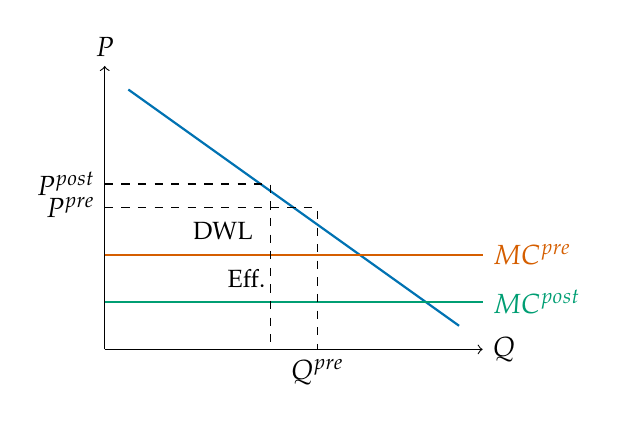
\begin{tikzpicture}[scale=0.6]
			% Axes
			\draw[->] (0,0) -- (8,0) node[right] {$Q$};
			\draw[->] (0,0) -- (0,6) node[above] {$P$};

			% Demand
			\draw[thick, blue] (0.5,5.5) -- (7.5,0.5);

			% Pre-merger MC
			\draw[thick, red] (0,2) -- (8,2) node[right] {$MC^{pre}$};

			% Post-merger MC (lower)
			\draw[thick, green] (0,1) -- (8,1) node[right] {$MC^{post}$};

			% Pre-merger price
			\draw[dashed] (0,3) -- (4.5,3) -- (4.5,0);
			\node[left] at (0,3) {$P^{pre}$};
			\node[below] at (4.5,0) {$Q^{pre}$};

			% Post-merger price
			\draw[dashed] (0,3.5) -- (3.5,3.5) -- (3.5,0);
			\node[left] at (0,3.5) {$P^{post}$};

			% Labels for areas
			\node at (2.5,2.5) {\small DWL};
			\node at (3,1.5) {\small Eff.};
		\end{tikzpicture}
	\end{center}
	\begin{wideitemize}
		\item DWL (lost surplus) vs Efficiency gain (cost savings)
		\item Merger is welfare-improving if Efficiency $>$ DWL
	\end{wideitemize}
\end{frame}

\begin{frame}{Practice: Merger policy}
	\begin{wideitemize}
		\item \textbf{Question:} Market has shares: 35\%, 25\%, 20\%, 15\%, 5\%.
		\item The 35\% and 25\% firms propose to merge.
		\item (a) Calculate pre-merger and post-merger HHI.
		\item (b) Would this merger likely face scrutiny under the Guidelines?
	\end{wideitemize}
	\vspace{10pt}
	\centering
	\textit{Take 3 minutes.}
\end{frame}

\begin{frame}{Practice: Merger policy (solution)}
	\begin{solutionbox}[Solution]
		\begin{wideitemize}
			\item \textbf{(a) Pre-merger:}
			\begin{align*}
				HHI = 35^2 + 25^2 + 20^2 + 15^2 + 5^2 = 2500
			\end{align*}
			\item \textbf{Post-merger:}
			\begin{align*}
				HHI = 60^2 + 20^2 + 15^2 + 5^2 = 4250
			\end{align*}
			\item $\Delta HHI = 1750$ (or: $2 \times 35 \times 25 = 1750$)
			\item \textbf{(b) Yes.} Post-merger HHI $> 2500$ (highly concentrated) and $\Delta HHI > 200$. Merger would likely face significant scrutiny.
		\end{wideitemize}
	\end{solutionbox}
\end{frame}

\begin{frame}{Remedies in merger review}
	\begin{wideitemize}
		\item \textbf{If merger raises concerns, agencies can:}
		\begin{wideenumerate}
			\vspace{5pt}
			\item Block the merger entirely
			\item Require divestitures (sell some products/plants)
			\item Impose behavioral conditions (licensing, access)
		\end{wideenumerate}
		\item \textbf{Divestitures:} Sell assets to maintain competition
		\begin{wideitemize}
			\vspace{5pt}
			\item Must sell to capable buyer
			\item Assets must be ``viable'' standalone
		\end{wideitemize}
		\item Example: T-Mobile/Sprint required divestiture to Dish
	\end{wideitemize}
\end{frame}

\begin{frame}{Recent merger cases}
	\begin{wideitemize}
		\item \textbf{Tech mergers:}
		\begin{wideitemize}
			\vspace{5pt}
			\item Google/Fitbit: wearables and data
			\item Microsoft/Activision: gaming
		\end{wideitemize}
		\item \textbf{Healthcare:}
		\begin{wideitemize}
			\vspace{5pt}
			\item Hospital mergers: quality vs price concerns
		\end{wideitemize}
		\item \textbf{Key issues in modern cases:}
		\begin{wideitemize}
			\vspace{5pt}
			\item Data as competitive asset
			\item Potential competition (would target have grown into competitor?)
			\item Vertical concerns (platforms buying content)
		\end{wideitemize}
	\end{wideitemize}
\end{frame}

\begin{frame}{Merger simulation vs HHI}
	\begin{center}
	\begin{tabular}{|l|p{4cm}|p{4cm}|}
		\hline
		& \textbf{HHI} & \textbf{Merger Simulation} \\
		\hline
		\textbf{Data needed} & Market shares & Demand estimates \\
		\hline
		\textbf{Output} & Concentration screen & Predicted price increase \\
		\hline
		\textbf{Pros} & Simple, transparent & Accounts for substitution \\
		\hline
		\textbf{Cons} & Ignores substitution & Requires demand model \\
		\hline
	\end{tabular}
	\end{center}
	\vspace{5pt}
	\begin{wideitemize}
		\item Modern merger review uses both approaches
	\end{wideitemize}
\end{frame}

\begin{frame}{Connection to HW2}
	\begin{wideitemize}
		\item \textbf{HW2 asks you to:}
		\begin{wideenumerate}
			\vspace{5pt}
			\item Take demand estimates (given)
			\item Compute pre-merger margins and implied MC
			\item Change ownership matrix
			\item Solve for post-merger equilibrium
			\item Calculate price effects and welfare change
		\end{wideenumerate}
		\item This connects Part 1 (demand) to Part 2 (competition)
		\item Same methodology used in real merger cases!
	\end{wideitemize}
\end{frame}

\begin{frame}{Merger analysis summary}
	\begin{wideenumerate}
		\item \textbf{Diversion ratio:} Key determinant of price effects
		\begin{wideitemize}
			\vspace{3pt}
			\item High diversion = close substitutes = larger price increase
		\end{wideitemize}
		\item \textbf{Simulation:} Change ownership, solve new equilibrium
		\item \textbf{UPP:} Quick screen: $D \times margin$
		\item \textbf{HHI:} Concentration screen, not definitive
		\item \textbf{Efficiencies:} Can offset price effects, but hard to prove
		\item \textbf{Practice:} Apply these tools in HW2!
	\end{wideenumerate}
\end{frame}

%%%%%%%%%%%%%%%%%%%%%%%%%%%%%%%%%%%%%%%%%%%%%%%%%%%%%%%%%%%%%
% KEY POINTS
%%%%%%%%%%%%%%%%%%%%%%%%%%%%%%%%%%%%%%%%%%%%%%%%%%%%%%%%%%%%%

\begin{frame}{Key Points}
	\vspace{11pt}
	\begin{wideenumerate}
		\item Mergers reduce competition by \textbf{internalizing substitution}
		\item \textbf{Merger simulation:} Use demand + ownership change to predict prices
		\item Key: ownership matrix $\mathbf{H}$ changes from 0 to 1 for merged products
		\item FOC changes: merged firm counts cross-price effects
		\item \textbf{SSNIP test:} Would hypothetical monopolist raise price 5\%?
		\item \textbf{HHI} = $\Sigma s_i^2 \times 10000$; $\Delta HHI$ screens mergers
		\item \textbf{Efficiency defense:} Cost savings may offset price effects
	\end{wideenumerate}
\end{frame}

\begin{frame}{Next time}
	\begin{wideitemize}
		\item \textbf{Lecture 11:} Vertical Relationships
		\begin{wideitemize}
			\vspace{5pt}
			\item Double marginalization
			\item Vertical integration
			\item Vertical restraints (RPM, exclusive dealing)
		\end{wideitemize}
	\end{wideitemize}
\end{frame}

\end{document}
